\documentclass[11pt,fleqn]{article}
\usepackage{../cs188,latexsym,epsf, amsmath,amsfonts,graphicx,url,multicol}
\usepackage{caption}
\usepackage{subcaption}
\lecture{4}
\def\title{Note \the\lecturenumber}
\begin{document}
\maketitle


\iffalse
\documentclass[11pt,fleqn]{article}
\usepackage{latexsym,epsf,amsmath,amsfonts,graphicx,url}

\title{Note 4}

\newcommand{\F}{\mathbb{F}}
\newcommand{\Z}{\mathbb{Z}}
\newcommand{\Q}{\mathbb{Q}}
\newcommand{\R}{\mathbb{R}}
\newcommand{\C}{\mathbb{C}}

\begin{document}

\maketitle
\fi

\section*{Non-Deterministic Search}
Picture a runner, coming to the end of his first ever marathon. Though it seems likely he will complete the race and claim the accompanying everlasting glory, it's by no means guaranteed. He may pass out from exhaustion or misstep and slip and fall, tragically breaking both of his legs. Even more unlikely, a literally earth-shattering earthquake may spontaneously occur swallow up the runner mere inches before he crosses the finish line. Such possibilities add a degree of \textit{uncertainty} to the runner's actions, and it's this uncertainty that will be the subject of the following discussion. In the first note, we talked about traditional search problems and how to solve them; then, in the third note, we changed our model to account for adversaries and other agents in the world that influenced our path to goal states. Now, we'll change our model again to account for another influencing factor - the dynamics of world itself. The environment in which an agent is placed may subject the agent's actions to being \textbf{nondeterministic}. This is, in fact, the case in many card games such as poker or blackjack, where there exists an inherent uncertainty from the randomness of card dealing. Such problems where the world poses a degree of uncertainty are known as \textbf{nondeterministic search problems}, and can be solved with models known as \textbf{Markov decision processes}, or MDPs.

\section*{Markov Decision Processes}
A Markov Decision Process is defined by several properties:
\vspace{-2.5mm}
\begin{itemize}
	\item A set of states $S$. States in MDPs are represented in the same way as states in traditional search problems.
	\item A set of actions $A$. Actions in MDPs are also represented in the same way as in traditional search problems.
	\item A start state.
	\item Possibly one or more terminal states.
	\item Possibly a \textbf{discount factor} $\gamma$. We'll cover discount factors shortly.
	\item A \textbf{transition function} $T(s, a, s')$. Since we have introduced the possibility of nondeterministic actions, we need a way to delineate the likelihood of the possible outcomes after taking any given action from any given state. The transition function for a MDP does exactly this - it's a probability function which represents the probability that an agent taking an action $a \in A$ from a state $s \in S$ ends up in a state $s' \in S$.
	\item A \textbf{reward function} $R(s, a, s')$. Typically, MDPs are modeled with small "living" rewards at each step to reward an agent's survival, along with large rewards for arriving at a terminal state. Rewards may be positive or negative depending on whether or not they benefit the agent in question, and the agent's objective is naturally to acquire the maximum reward possible before arriving at some terminal state.
\end{itemize}
Constructing a MDP for a situation is quite similar to constructing a state-space graph for a search problem, with a couple additional caveats. Consider the motivating example of a racecar: 
\begin{center}
	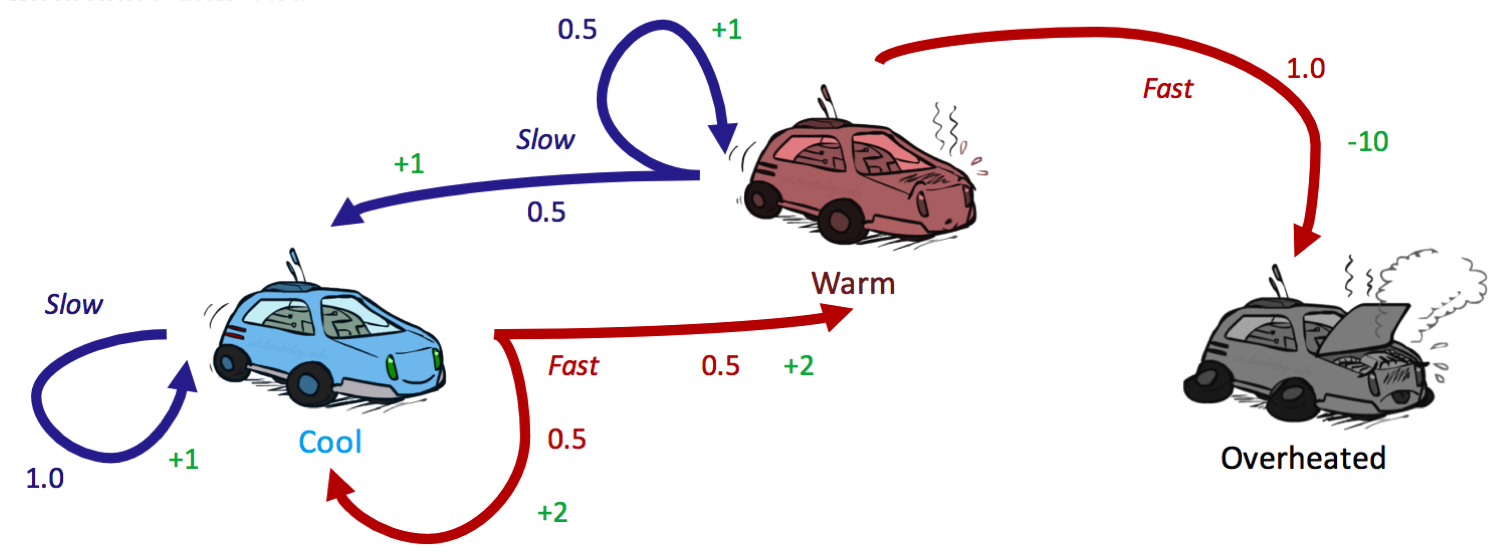
\includegraphics[width=15cm]{img/race-car}
\end{center}
There are three possible states, $S = \{cool, warm, overheated\}$, and two possible actions $A = \{slow, fast\}$. Just like in a state-space graph, each of the three states is represented by a node, with edges representing actions. $Overheated$ is a terminal state, since once a racecar agent arrives at this state, it can no longer perform any actions for further rewards (it's a \textit{sink state} in the MDP and has no outgoing edges). Notably, for nondeterministic actions, there are multiple edges representing the same action from the same state with differing successor states. Each edge is annotated not only with the action it represents, but also a transition probability and corresponding reward. These are summarized below:
\begin{multicols}{2}
\begin{itemize}
\item{\textbf{Transition Function}: $\:\: T(s, a, s')$}
	\begin{itemize}
		\item $T(cool, slow, cool) = 1$
		\item $T(warm, slow, cool) = 0.5$
		\item $T(warm, slow, warm) = 0.5$
		\item $T(cool, fast, cool) = 0.5$
		\item $T(cool, fast, warm) = 0.5$
		\item $T(warm, fast, overheated) = 1$
	\end{itemize}
\item{\textbf{Reward Function}: $\:\: R(s, a, s')$}
	\begin{itemize}
		\item $R(cool, slow, cool) = 1$
		\item $R(warm, slow, cool) = 1$
		\item $R(warm, slow, warm) = 1$
		\item $R(cool, fast, cool) = 2$
		\item $R(cool, fast, warm) = 2$
		\item $R(warm, fast, overheated) = -10$
	\end{itemize}
\end{itemize}
\end{multicols} 
\vspace{-2.5mm}
 We represent the movement of an agent through different MDP states over time with discrete \textbf{timesteps}, defining $s_t \in S$ and $a_t \in A$ as the state in which an agent exists and the action which an agent takes at timestep $t$ respectively. An agent starts in state $s_0$ at timestep 0, and takes an action at every timestep. The movement of an agent through a MDP can thus be modeled as follows:
$$s_0 \xrightarrow{a_0} s_1 \xrightarrow{a_1} s_2 \xrightarrow{a_2} s_3 \xrightarrow{a_3}...$$
Additionally, knowing that an agent's goal is to maximize it's reward across all timesteps, we can correspondingly express this mathematically as a maximization of the following utility function:
$$U([s_0, a_0, s_1, a_1, s_2, ...]) = R(s_0, a_0, s_1) + R(s_1, a_1, s_2) + R(s_2, a_2, s_3) + ...$$
Markov decision processes, like state-space graphs, can be unraveled into search trees. Uncertainty is modeled in these search trees with \textbf{q-states}, also known as \textbf{action states}, essentially identical to expectimax chance nodes. This is a fitting choice, as q-states use probabilities to model the uncertainty that the environment will land an agent in a given state just as expectimax chance nodes use probabilities to model the uncertainty that adversarial agents will land our agent in a given state through the move these agents select. The q-state represented by having taken action $a$ from state $s$ is notated as the tuple $(s, a)$.

Observe the unraveled search tree for our racecar, truncated to depth-2:
\begin{center}
	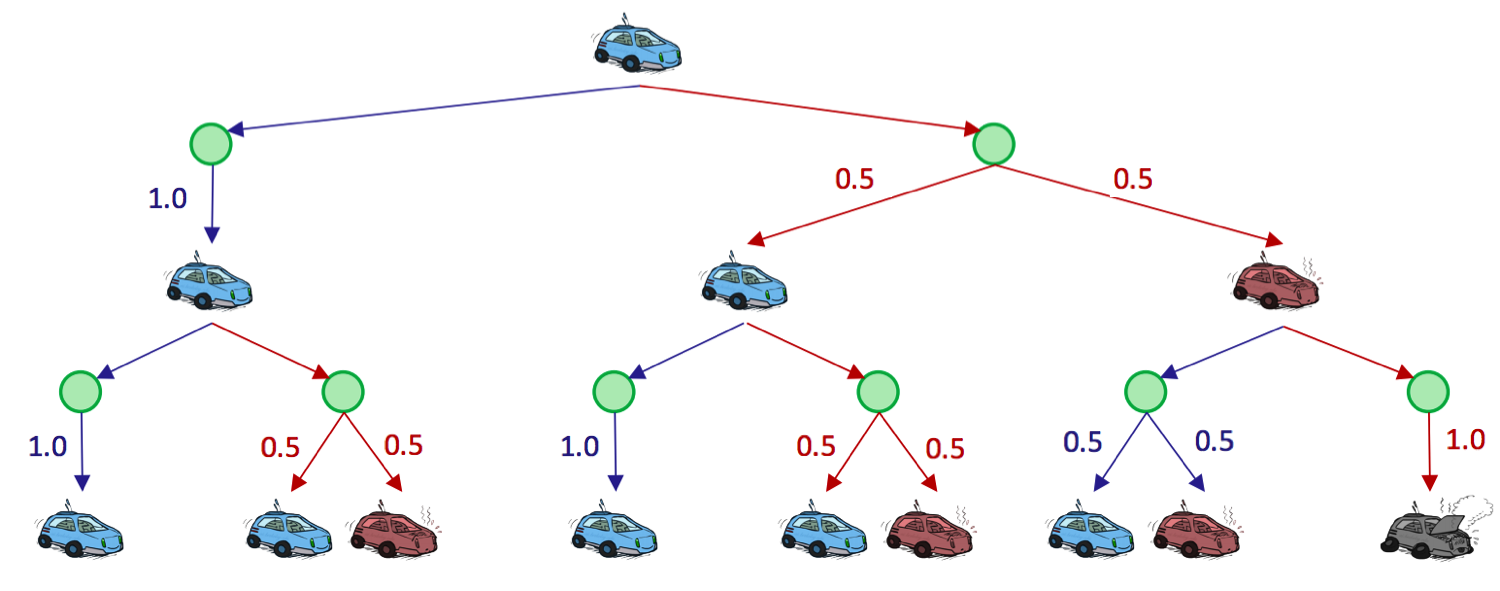
\includegraphics[width=15cm]{img/rc-search-tree}
\end{center}
The green nodes represent q-states, where an action has been taken from a state but has yet to be resolved into a successor state. It's important to understand that agents spend zero timesteps in q-states, and that they are simply a construct created for ease of representation and development of MDP algorithms.

\subsection*{Finite Horizons and Discounting}
There is an inherent problem with our racecar MDP - we haven't placed any time constraints on the number of timesteps for which a racecar can take actions and collect rewards. With our current formulation, it could routinely choose $a = slow$ at every timestep forever, safely and effectively obtaining infinite reward without any risk of overheating. This is prevented by the introduction of \textbf{finite horizons} and/or \textbf{discount factors}. An MDP enforcing a finite horizon is simple - it essentially defines a "lifetime" for agents, which gives them some set number of timesteps $n$ to accrue as much reward as they can before being automatically terminated. We'll return to this concept shortly.

Discount factors are slightly more complicated, and are introduced to model an exponential decay in the value of rewards over time. Concretely, with a discount factor of $\gamma$, taking action $a_t$ from state $s_t$ at timestep $t$ and ending up in state $s_{t+1}$ results in a reward of $\gamma^t R(s_t, a_t, s_{t+1})$ instead of just $R(s_t, a_t, s_{t+1})$. Now, instead of maximizing the \textbf{additive utility} 
$$U([s_0, a_0, s_1, a_1, s_2, ...]) = R(s_0, a_0, s_1) + R(s_1, a_1, s_2) + R(s_2, a_2, s_3) + ...$$ 
we attempt to maximize \textbf{discounted utility}
$$U([s_0, a_0, s_1, a_1, s_2, ...]) = R(s_0, a_0, s_1) + \gamma R(s_1, a_1, s_2) + \gamma^2 R(s_2, a_2, s_3) + ...$$
Noting that the above definition of a discounted utility function looks dangerously close to a \textbf{geometric series} with ratio $\gamma$, we can prove that it's guaranteed to be finite-valued as long as the constraint $|\gamma| < 1$ (where $|n|$ denotes the absolute value operator) is met through the following logic:
\begin{eqnarray*}
	U([s_0, s_1, s_2, ...]) &=& R(s_0, a_0, s_1) + \gamma R(s_1, a_1, s_2) + \gamma^2 R(s_2, a_2, s_3) + ... \\
	&=& \sum_{t=0}^{\infty} \gamma^t R(s_t, a_t, s_{t+1})
	\leq \sum_{t=0}^{\infty} \gamma^t R_{max}
	= \boxed{\frac{R_{max}}{1 - \gamma}}
\end{eqnarray*}
where $R_{max}$ is the maximum possible reward attainable at any given timestep in the MDP. Typically, $\gamma$ is selected strictly from the range $0 < \gamma < 1$ since values values in the range $-1 < \gamma \leq 0$ are simply not meaningful in most real-world situations - a negative value for $\gamma$ means the reward for a state $s$ would flip-flop between positive and negative values at alternating timesteps.

\subsection*{Markovianess}
Markov decision processes are "markovian" in the sense that they satisfy the \textbf{Markov property}, or \textbf{memoryless property}, which states that the present is independent of both the future and the past. To express this mathematically, consider an agent that has visited states $s_0, s_1, ..., s_t$ after taking actions $a_0, a_1, ..., a_{t-1}$ in some MDP, and has just taken action $a_t$. The probability that this agent then arrives at state $s_{t+1}$ given their history of previous states visited and actions taken can be written as follows:
$$P(S_{t+1} = s_{t+1} | S_t = s_t, A_t = a_t, S_{t-1} = s_{t-1}, A_{t-1} = a_{t-1}, ..., S_0 = s_0)$$
where each $S_t$ denotes the random variable representing our agent's state and $A_t$ denotes the random variable representing the action our agent takes at time $t$. The Markov property states that the above probability can be simplified as follows:
$$P(S_{t+1} = s_{t+1} | S_t = s_t, A_t = a_t, S_{t-1} = s_{t-1}, A_{t-1} = a_{t-1}, ..., S_0 = s_0) = P(S_{t+1} = s_{t+1} | S_t = s_t, A_t = a_t)$$
which is "memoryless" in the sense that the probability of arriving in a state $s'$ at time $t+1$ depends only on the state $s$ and action $a$ taken at time $t$, not on any earlier states or actions. In fact, it is these memoryless probabilities which are encoded by the transition function: $\boxed{T(s, a, s') = P(s' | s, a)}$.

\section*{Solving Markov Decision Processes}
Recall that in deterministic, non-adversarial search, solving a search problem means finding an optimal plan to arrive at a goal state. Solving a Markov decision process, on the other hand, means finding an optimal \textbf{policy} $\pi^*: S \rightarrow A$, a function mapping each state $s \in S$ to an action $a \in A$. An explicit policy $\pi$ defines a reflex agent - given a state $s$, an agent at $s$ implementing $\pi$ will select $a = \pi(s)$ as the appropriate action to make without considering future consequences of its actions. An optimal policy is one that if followed by the implementing agent, will yield the maximum expected total reward or utility.

Consider the following MDP with $S = \{a, b, c, d, e\}$, $A = \{East, West, Exit\}$ (with $Exit$ being a valid \\ action only in states $a$ and $e$ and yielding rewards of 10 and 1 respectively), a discount factor $\gamma = 0.1$, and deterministic transitions:
\begin{center}
	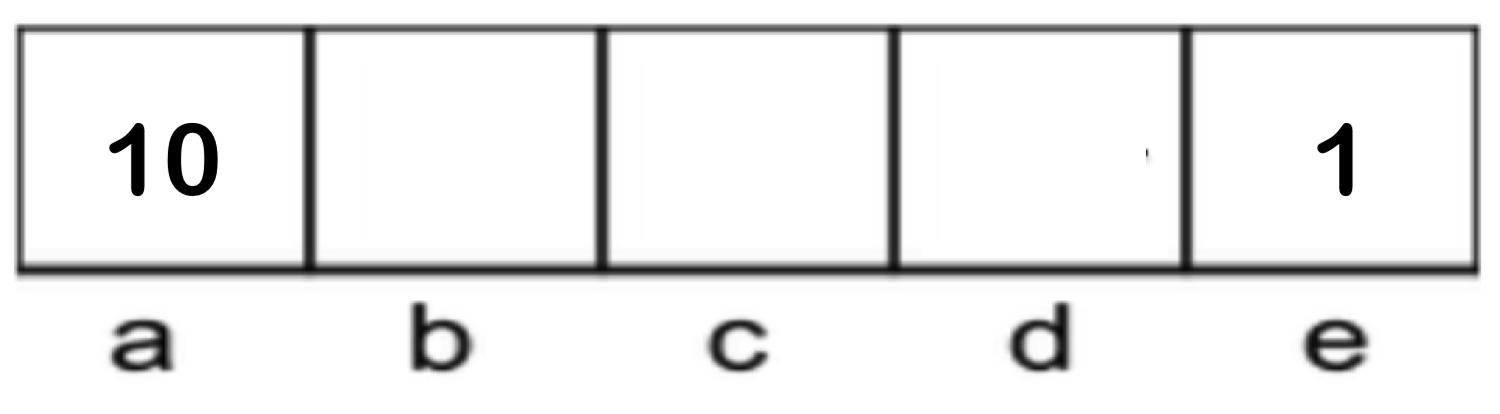
\includegraphics[width=6cm]{img/easy-mdp}
\end{center}
\newpage
Two potential policies for this MDP are as follows:
\begin{center}
\begin{figure}[!h]
\centering
\begin{subfigure}{.5\textwidth}
  \centering
  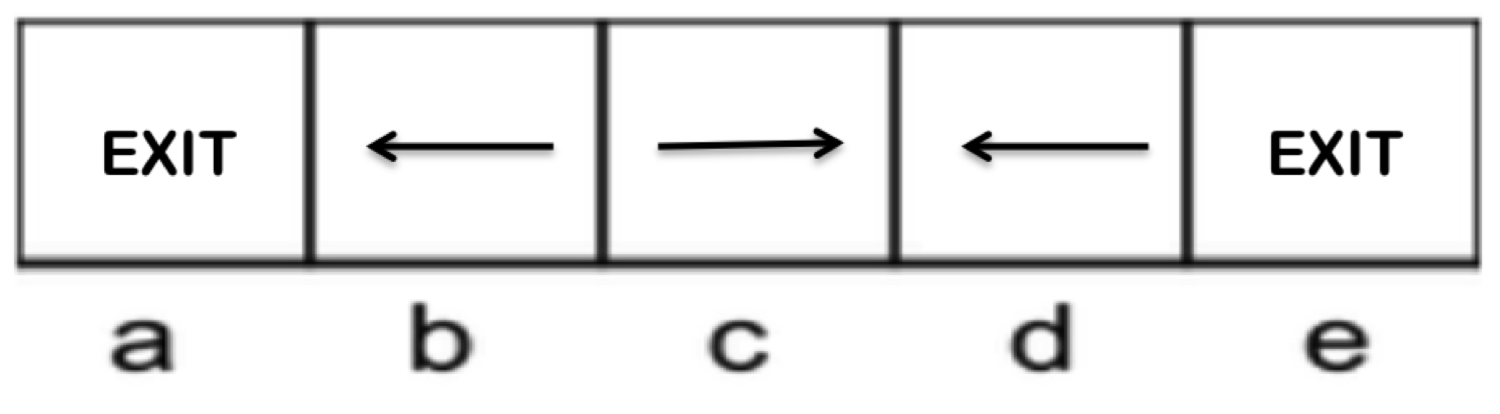
\includegraphics[width=6cm]{img/policy-1}
  \caption{Policy 1}
  \label{fig:sub1}
\end{subfigure}%
\begin{subfigure}{.5\textwidth}
  \centering
  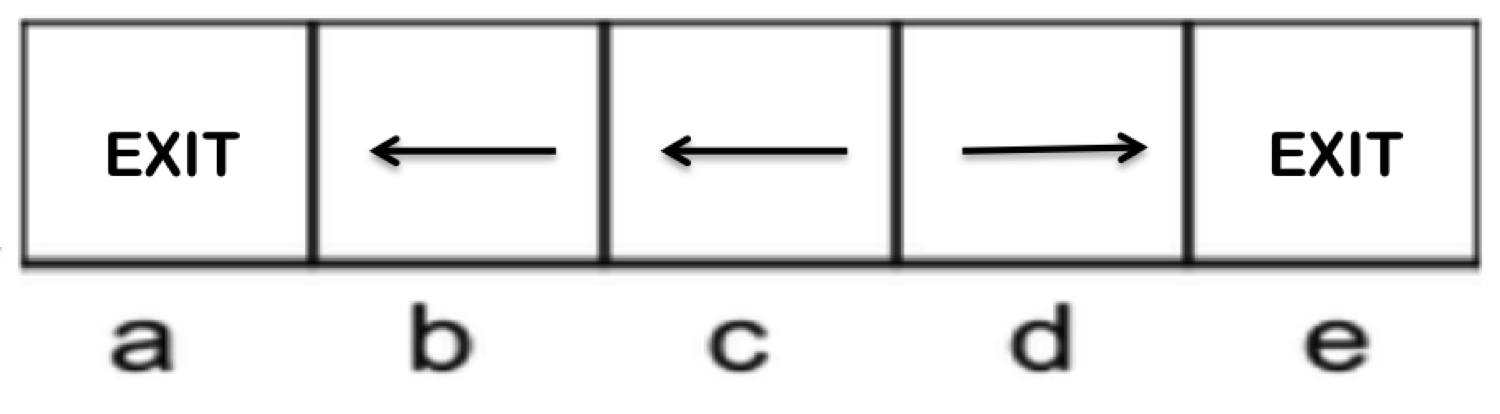
\includegraphics[width=6cm]{img/policy-2}
  \caption{Policy 2}
  \label{fig:sub2}
\end{subfigure}
\label{fig:test}
\end{figure}
\end{center}
With some investigation, it's not hard to determine that Policy 2 is optimal. Following the policy until making action $a = Exit$ yields the following rewards for each start state:
\begin{center}
\begin{tabular}{ |c|c|c| } 
 \hline
 \textbf{Start State} & \textbf{Reward} \\ 
 \hline
 a & 10 \\ 
 \hline
 b & 1 \\ 
 \hline
 c & 0.1 \\ 
 \hline
 d & 0.1 \\ 
 \hline
 e & 1 \\
 \hline
\end{tabular}
\end{center}

We'll now learn how to solve such MDPs (and much more complex ones!) algorithmically using the \\ \textbf{Bellman equation} for Markov decision processes.

\subsection*{The Bellman Equation}
In order to talk about the Bellman equation for MDPs, we must first introduce two new mathematical quantities:
\begin{itemize}
	\item The optimal value of a state $s$, $V^*(s)$ - the optimal value of $s$ is the expected value of the utility an optimally-behaving agent that starts in $s$ receives .
	\item The optimal value of a q-state $(s, a)$, $Q^*(s, a)$ - the optimal value of $(s, a)$ is the expected value of the utility an agent receives after starting in $s$, taking $a$, and acting optimally henceforth. 
\end{itemize} 
Using these two new quantities and the other MDP quantities discussed earlier, the Bellman equation is defined as follows:
$$V^*(s) = \max_a \sum_{s'}T(s, a, s')[R(s, a, s') + \gamma V^*(s')]$$
Before we begin interpreting what this means, let's also define the equation for the optimal value of a q-state (more commonly known as an optimal \textbf{q-value}):
$$Q^*(s, a) = \sum_{s'}T(s, a, s')[R(s, a, s') + \gamma V^*(s')]$$
Note that this second definition allows us to reexpress the Bellman equation as
$$V^*(s) = \max_a Q^*(s, a)$$
which is a dramatically simpler quantity. The Bellman equation is an example of a \textit{dynamic programming equation}, an equation that decomposes a problem into smaller subproblems via an inherent recursive structure. We can see this inherent recursion in the equation for the q-value of a state, in the term $[R(s, a, s') + \gamma V^*(s')]$. This term represents the total utility an agent receives by first taking $a$ from $s$ and arriving at $s'$ and then acting optimally henceforth - $R(s, a, s')$ added to the optimal reward attainable from $s'$, $V^*(s')$, which is discounted by $\gamma$ to account for the passage of the timestep in taking $a$. Though in most cases there exists a vast number of possible sequences of states and actions from $s'$ to some terminal state, all this detail is abstracted away and encapsulated in a single recursive value, $V^*(s')$.

We can now take another step outwards and consider the full equation for q-value. Knowing $[R(s, a, s') + \gamma V^*(s')]$ represents the utility attained by acting optimally after arriving in state $s'$ from q-state $(s, a)$, it becomes evident that the quantity
$$\sum_{s'}T(s, a, s')[R(s, a, s') + \gamma V^*(s')]$$
is simply a weighted sum of utilities, with each utility weighted by its probability of occurrence. This is definitionally the \textit{expected utility} of acting optimally from q-state $(s, a)$ onwards! This completes our analysis and gives us enough insight to interpret the full Bellman equation - the optimal value of a state, $V^*(s)$, is simply the \textit{maximum expected utility} over all possible actions from $s$. Computing maximum expected utility for a state $s$ is essentially the same as running expectimax - we first compute the expected utility from each q-state $(s, a)$ (equivalent to computing the value of chance nodes), then compute the maximum over these nodes to compute the maximum expected utility (equivalent to computing the value of a maximizer node).

One final note on the Bellman equation - it's usage is as a \textit{condition} for optimality. In other words, if we can somehow determine a value $V(s)$ for every state $s \in S$ such that the Bellman equation holds true for each of these states, we can conclude that these values are the optimal values for their respective states. Indeed, satisfying this condition implies $\forall s \in S, \:\: V(s) = V^*(s)$.

\subsection*{Value Iteration}
Now that we have a framework to test for optimality of the values of states in a MDP, the natural follow-up question to ask is how to actually compute these optimal values. To answer this question, we need \textbf{time-limited values} (the natural result of enforcing finite horizons). The time-limited value for a state $s$ with a time-limit of $k$ timesteps is denoted $V_k(s)$, and represents the maximum expected utility attainable from $s$ given that the Markov decision process under consideration terminates in $k$ timesteps.  Equivalently, this is what a depth-$k$ expectimax run on the search tree for a MDP returns.

\textbf{Value iteration} is a \textbf{dynamic programming algorithm} that uses an iteratively longer time limit to compute time-limited values until convergence. It operates as follows:
\begin{enumerate}
	\item $\forall s \in S,$ initialize $V_0(s) = 0$. This should be intuitive, since setting a time limit of 0 timesteps means no actions can be taken before termination, and so no rewards can be acquired.
	\item Repeat the following update rule until convergence:
		$$\forall s \in S, \:\: V_{k+1}(s) \leftarrow \max_a \sum_{s'}T(s, a, s')[R(s, a, s') + \gamma V_k(s')]$$
		At iteration $k$ of value iteration, we use the time-limited values for with limit $k$ for each state to generate the time-limited values with limit $(k+1)$. In essence, we use computed solutions to subproblems (all the $V_k(s)$) to iteratively build up solutions to larger subproblems (all the $V_{k+1}(s)$); this is what makes value iteration a dynamic programming algorithm. 
\end{enumerate}

Note that though the Bellman equation looks essentially identical in construction to the update rule above, they are not the same. One is a condition for optimality, while the other uses that condition to iteratively update values until convergence, at which point $\forall s \in S, \:\: V_k(s) = V_{k+1}(s) = V^*(s)$.
\newpage
Let's see a few updates of value iteration in practice by revisiting our racecar MDP from earlier, introducing a discount factor of $\gamma = 0.5$:
\begin{center}
	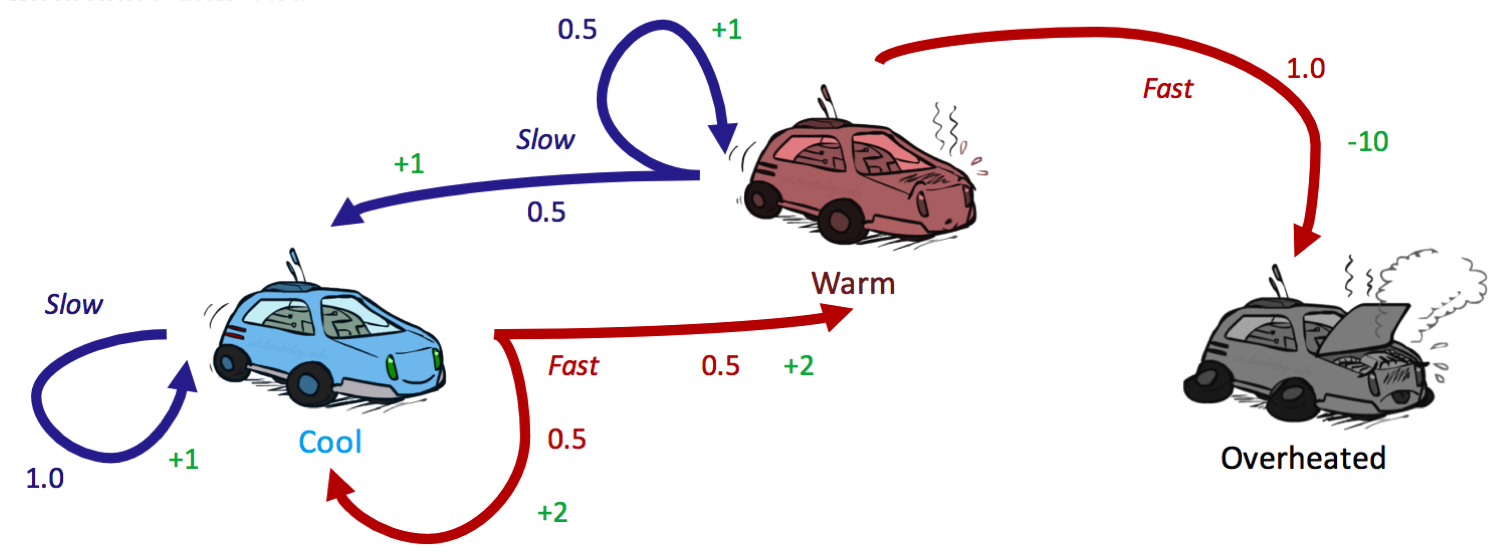
\includegraphics[width=15cm]{img/race-car}
\end{center}

We begin value iteration by initialization of all $V_0(s) = 0$:
\begin{center}
\begin{tabular}{ |c|c|c|c| } 
 \hline
  & \textbf{cool} & \textbf{warm} & \textbf{overheated} \\ 
 \hline
 $V_0$ & 0 & 0 & 0 \\
 \hline
\end{tabular}
\end{center}
In our first round of updates, we can compute $\forall s \in S, \:\: V_1(s)$ as follows:
\begin{eqnarray*}
	V_1(cool) &=& \max\{1 \cdot [1 + 0.5 \cdot 0],\:\: 0.5 \cdot [2 + 0.5 \cdot 0] + 0.5 \cdot [2 + 0.5 \cdot 0]\} \\
	&=& \max\{1, 2\} \\
	&=& \boxed{2} \\
	V_1(warm) &=& \max\{0.5 \cdot [1 + 0.5 \cdot 0] + 0.5 \cdot [1 + 0.5 \cdot 0],\:\: 1 \cdot [-10 + 0.5 \cdot 0]\} \\
	&=& \max\{1, -10\} \\
	&=& \boxed{1} \\
	V_1(overheated) &=& \max\{\} \\
	&=& \boxed{0}
\end{eqnarray*}
\begin{center}
\begin{tabular}{ |c|c|c|c| } 
 \hline
  & \textbf{cool} & \textbf{warm} & \textbf{overheated} \\ 
 \hline
 $V_0$ & 0 & 0 & 0 \\
 \hline
 $V_1$ & 2 & 1 & 0 \\
 \hline
\end{tabular}
\end{center}
Similarly, we can repeat the procedure to compute a second round of updates with our newfound values for $V_1(s)$ to compute $V_2(s)$.
\begin{eqnarray*}
	V_2(cool) &=& \max\{1 \cdot [1 + 0.5 \cdot 2],\:\: 0.5 \cdot [2 + 0.5 \cdot 2] + 0.5 \cdot [2 + 0.5 \cdot 1]\} \\
	&=& \max\{2, 2.75\} \\
	&=& \boxed{2.75} \\
	V_2(warm) &=& \max\{0.5 \cdot [1 + 0.5 \cdot 2] + 0.5 \cdot [1 + 0.5 \cdot 1],\:\: 1 \cdot [-10 + 0.5 \cdot 0]\} \\
	&=& \max\{1.75, -10\} \\
	&=& \boxed{1.75} \\
	V_2(overheated) &=& \max\{\} \\
	&=& \boxed{0}
\end{eqnarray*}
\begin{center}
\begin{tabular}{ |c|c|c|c| } 
 \hline
  & \textbf{cool} & \textbf{warm} & \textbf{overheated} \\ 
 \hline
 $V_0$ & 0 & 0 & 0 \\
 \hline
 $V_1$ & 2 & 1 & 0 \\
 \hline
 $V_2$ & 2.75 & 1.75 & 0 \\
 \hline
\end{tabular}
\end{center}
It's worthwhile to observe that $V^*(s)$ for any terminal state must be 0, since no actions can ever be taken from any terminal state to reap any rewards.

\subsection*{Policy Extraction}
Recall that our ultimate goal in solving a MDP is to determine an optimal policy. This can be done once all optimal values for states are determined using a method called \textbf{policy extraction}. The intuition behind policy extraction is very simple: if you're in a state $s$, you should take the action $a$ which yields the maximum expected utility. Not surprisingly, $a$ is the action which takes us to the q-state with maximum q-value, allowing for a formal definition of the optimal policy:
$$\forall s \in S, \:\: \pi^*(s) = \underset{a}{\operatorname{argmax}}\: Q^*(s, a) = \underset{a}{\operatorname{argmax}}\: \sum_{s'}T(s, a, s')[R(s, a, s') + \gamma V^*(s')]$$
It's useful to keep in mind for performance reasons that it's better for policy extraction to have the optimal q-values of states, in which case a single ${\operatorname{argmax}}$ operation is all that is required to determine the optimal action from a state. Storing only each $V^*(s)$ means that we must recompute all necessary q-values with the Bellman equation before applying ${\operatorname{argmax}}$, equivalent to performing a depth-$1$ expectimax.

\subsection*{Policy Iteration}
Value iteration can be quite slow. At each iteration, we must update the values of all $|S|$ states (where $|n|$ refers to the cardinality operator), each of which requires iteration over all $|A|$ actions as we compute the q-value for each action. The computation of each of these q-values, in turn, requires iteration over each of the $|S|$ states again, leading to a poor runtime of $O(|S|^2|A|)$. Additionally, when all we want to determine is the optimal policy for the MDP, value iteration tends to do a lot of overcomputation since the policy as computed by policy extraction generally converges significantly faster than the values themselves. The fix for these flaws is to use \textbf{policy iteration} as an alternative, an algorithm that maintains the optimality of value iteration while providing significant performance gains. Policy iteration operates as follows:
\begin{enumerate}
	\item Define an \textit{initial policy}. This can be arbitrary, but policy iteration will converge faster the closer the initial policy is to the eventual optimal policy.
	\item Repeat the following until convergence:
		\begin{itemize}
			\item Evaluate the current policy with \textbf{policy evaluation}. For a policy $\pi$, policy evaluation means computing $V^{\pi}(s)$ for all states $s$, where $V^{\pi}(s)$ is expected utility of starting in state $s$ when following $\pi$:
				$$V^{\pi}(s) = \sum_{s'}T(s, \pi(s), s')[R(s, \pi(s), s') + \gamma V^{\pi}(s')]$$
			Define the policy at iteration $i$ of policy iteration as $\pi_i$. Since we are fixing a single action for each state, we no longer need the $\max$ operator which effectively leaves us with a system of $|S|$ equations generated by the above rule. Each $V^{\pi_i}(s)$ can then be computed by simply solving this system.
			Alternatively, we can also compute $V^{\pi_i}(s)$ by using the following update rule until convergence, just like in value iteration:
				$$V^{\pi_i}_{k+1}(s) \leftarrow \sum_{s'}T(s, \pi_i(s), s')[R(s, \pi_i(s), s') + \gamma V^{\pi_i}_k(s')]$$
			However, this second method is typically slower in practice.
			\item Once we've evaluated the current policy, use \textbf{policy improvement} to generate a better policy. Policy improvement uses policy extraction on the values of states generated by policy evaluation to generate this new and improved policy:
				$$\pi_{i+1}(s) = \underset{a}{\operatorname{argmax}}\: \sum_{s'}T(s, a, s')[R(s, a, s') + \gamma V^{\pi_i}(s')]$$ 
			If $\pi_{i+1} = \pi_i$, the algorithm has converged, and we can conclude that $\pi_{i+1} = \pi_i = \pi^*$.
		\end{itemize}
\end{enumerate}

Let's run through our racecar example one last time (getting tired of it yet?) to see if we get the same policy using policy iteration as we did with value iteration:

\begin{center}
	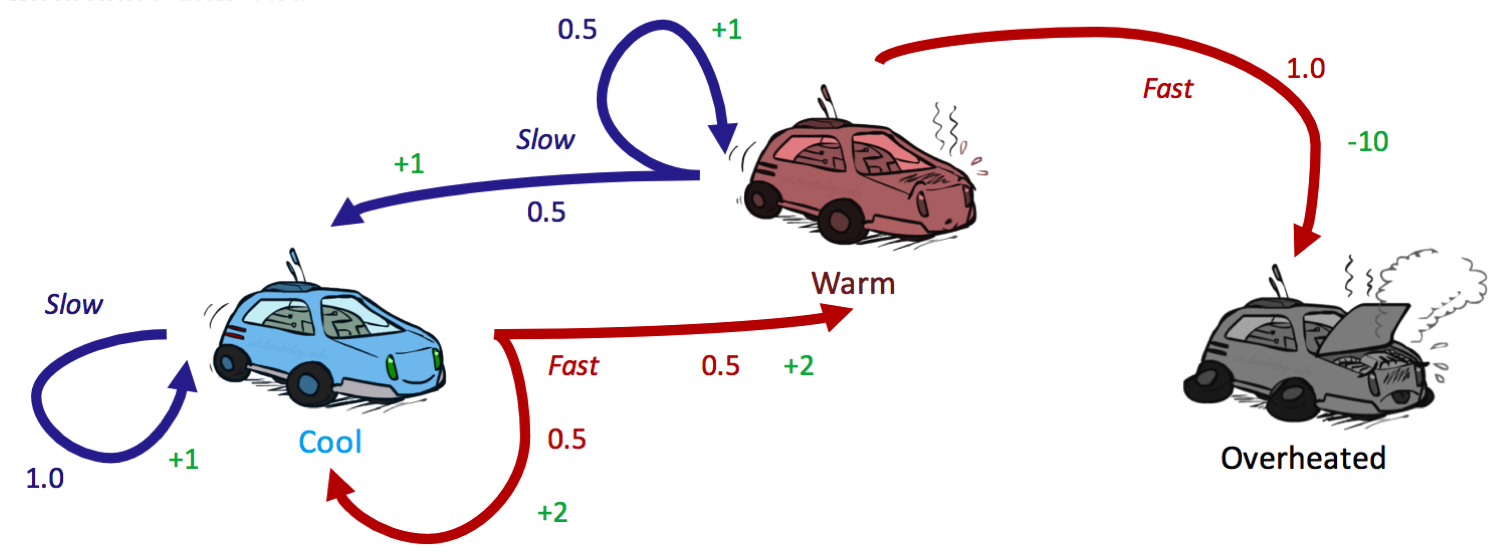
\includegraphics[width=15cm]{img/race-car}
\end{center}

We start with an initial policy of \textit{Always go slow}:
\begin{center}
\begin{tabular}{ |c|c|c|c| } 
 \hline
  & \textbf{cool} & \textbf{warm} & \textbf{overheated} \\ 
 \hline
 $\pi_0$ & $slow$ & $slow$ & $-$ \\
 \hline
\end{tabular}
\end{center}
Because terminal states have no outgoing actions, no policy can assign a value to one. Hence, it's reasonable to disregard the state $overheated$ from consideration as we have done, and simply assign $\forall i, \:\: V^{\pi_i}(s) = 0$ for any terminal state $s$. The next step is to run a round of policy evaluation on $\pi_0$:
\begin{eqnarray*}
	V^{\pi_0}(cool) &=& 1 \cdot [1 + 0.5 \cdot V^{\pi_0}(cool)] \\
	V^{\pi_0}(warm) &=& 0.5 \cdot [1 + 0.5 \cdot V^{\pi_0}(cool)]
					+ 0.5 \cdot [1 + 0.5 \cdot V^{\pi_0}(warm)] 
\end{eqnarray*}
Solving this system of equations for $V^{\pi_0}(cool)$ and $V^{\pi_0}(warm)$ yields:
\begin{center}
\begin{tabular}{ |c|c|c|c| } 
 \hline
  & \textbf{cool} & \textbf{warm} & \textbf{overheated} \\ 
 \hline
 $V^{\pi_0}$ & 2 & 2 & 0 \\
 \hline
\end{tabular}
\end{center}
We can now run policy extraction with these values:
\begin{eqnarray*}
	\pi_{1}(cool) &=& {\operatorname{argmax}}\{slow: 1 \cdot [1 + 0.5 \cdot 2],\:\: fast: 0.5 \cdot [2 + 0.5 \cdot 2] + 0.5 \cdot [2 + 0.5 \cdot 2]\} \\
				  &=& {\operatorname{argmax}}\{slow: 2,\:\: fast: 3\} \\
				  &=& \boxed{fast} \\
	\pi_{1}(warm) &=& {\operatorname{argmax}}\{slow: 0.5 \cdot [1 + 0.5 \cdot 2] + 0.5 \cdot [1 + 0.5 \cdot 2] ,\:\: fast: 1 \cdot [-10 + 0.5 \cdot 0]\} \\
		  		  &=& {\operatorname{argmax}}\{slow: 3,\:\: fast: -10\} \\
		  		  &=& \boxed{slow} 
\end{eqnarray*}
Running policy iteration for a second round yields $\pi_2(cool) = fast$ and $\pi_2(warm) = slow$. Since this is the same policy as $\pi_1$, we can conclude that $\pi_1 = \pi_2 = \pi^*$. Verify this for practice!
\begin{center}
\begin{tabular}{ |c|c|c|c| } 
 \hline
  & \textbf{cool} & \textbf{warm} \\ 
 \hline
 $\pi_0$ & $slow$ & $slow$ \\
 \hline
 $\pi_1$ & $fast$ & $slow$ \\
 \hline
 $\pi_2$ & $fast$ & $slow$ \\
 \hline
\end{tabular}
\end{center}
This example shows the true power of policy iteration: with only two iterations, we've already arrived at the optimal policy for our racecar MDP! This is more than we can say for when we ran value iteration on the same MDP, which was still several iterations from convergence after the two updates we performed.

\section*{Summary}
The material presented above has much opportunity for confusion. We covered value iteration, policy iteration, policy extraction, and policy evaluation, all of which look essentially the same, using the Bellman equation with subtle variation. All of these techniques use the Bellman equation towards the same purpose of obtaining an optimal policy. Below is a summary of when to use each algorithm:
	\begin{itemize}
		\item \textit{Value iteration}: Used for computing the optimal values of states with iterative convergence.
		\item \textit{Policy evaluation}: Used for computing the values of states under a specific policy.
		\item \textit{Policy extraction}: Used for determining a policy given the values of states, which may or may not be optimal (though optimal values yield an optimal policy).
		\item \textit{Policy iteration}: A technique that encapsulates both policy evaluation and policy extraction and is used for iterative convergence to an optimal policy. It tends to outperform value iteration, by virtue of the fact that policies usually converge must faster than the values of states.
	\end{itemize}
\end{document}